\begin{refsection}

\chapter{Neural Networks as Bayes Point Machines}\label{chap:bpm}

\begin{tcolorbox}
This chapter introduces a novel correspondence between neural networks and kernels. In particular, as both width and normalised margin are sent to infinity, the neural network function space concentrates on a particular kernel classifier. This kernel classifier aggregates over all infinitely wide neural networks that correctly classify the train sample. This offers a new, potentially fruitful perspective as to why neural networks generalise.
\end{tcolorbox}

Chapter \ref{chap:gp-pac-bayes} derived PAC-Bayes bounds for Gaussian process classification. These bounds may be readily transferred to neural networks---albeit infinitely wide ones---by leveraging the neural network--Gaussian process correspondence from Section \ref{sec:nngp}. Having these bounds is certainly nice, and they have been found to be non-vacuous \citep{seeger,Prez2020GeneralizationBF}. But what would be nicer is having the bounds inform some aspect of deep learning practice. For instance: could the bounds tell which single function should generalise best?

There is a problem, however. Theorem \ref{thm:pac-bayes-gpc} bounds the misclassification rate of the Gaussian process averaged over posterior draws. This leaves room for individual draws to generalise either significantly worse or significantly better than average. Then which single function should be returned in practice? 

To answer this question, the chapter takes a detour through \textit{Bayesian classification strategies}. A Bayesian classification strategy is a rule for combining an input $x$ with a posterior distribution $Q$ over classifiers to yield a prediction. The most natural of these strategies involve either randomly sampling a single posterior function or aggregating over the posterior. Bayesian wisdom, and also certain technical results \citep{lacasse}, suggest that aggregation over the posterior should perform best. This is for the simple reason that aggregation removes the variance incurred by sampling a posterior function. 

But the trouble with aggregation is that it is expensive. Naïvely, it involves either integrating or summing over lots of posterior functions. To get the benefits of aggregation without the associated cost, this chapter picks up on an old idea from the kernels literature.  A \textit{Bayes point machine} \citep{bpms} is a single posterior sample that, by itself, approximates the posterior aggregate. In the context of neural networks, this suggests the question:
\begin{quote}
    Can a single neural network report the aggregated classification of an ensemble of networks?
\end{quote}
Given the expressive power of the neural network function class, it might seem reasonable that the answer could be yes. In that case:
\begin{quote}
    How can such a network be found?
\end{quote}
This chapter attempts to resolve these two questions. The chapter argues that, in the limit of large width and large normalised margin, the entire space of neural networks that interpolate a training set \textit{concentrates} on a kernel classifier that itself aggregates over a posterior distribution. This implies that a single wide neural network trained to large normalised margin will attain the same reduction in the variance of its predictions as an aggregated Bayesian method.

\section{Bayesian classification strategies}

From a Bayesian perspective, there are three natural ways to use a posterior $Q$ over functions to classify a fresh input $x\in\mathcal{X}$. The first is the random strategy:
\begin{definition}[Gibbs classifier]
The \textit{Gibbs classifier} returns a random draw:
    \begin{equation}
        f_\mathrm{Gibbs}(x) \coloneqq \sign f(x)  \text{ for } f\sim Q.
    \end{equation}
\end{definition}
PAC-Bayes (Theorem \ref{thm:pac-bayes}) bounds the probability that the Gibbs classifier misclassifies a randomly drawn test point. But the Gibbs classifier, being random, has the misfortune of containing variance. A Bayesian would like to deal with this issue by integrating, or \textit{aggregating}, over the posterior, and thus removing this variance. This motivates the second strategy:
\begin{definition}[Bayes classifier]
The \textit{Bayes classifier} returns the majority vote:
    \begin{equation}
        f_\mathrm{Bayes}(x) \coloneqq \sign \Expect_{f\sim Q} \sign f(x).
    \end{equation}
\end{definition}
The majority is one form of aggregation. The third strategy employs another:
\begin{definition}[BPM classifier]
    The \textit{BPM classifier} returns the simple average:
        \begin{equation}
            f_\mathrm{BPM}(x) \coloneqq \sign \Expect_{f\sim Q} f(x).
        \end{equation}
\end{definition}

The abbreviation BPM is short for \textit{Bayes point machine}. Two observations motivate this terminology:
\begin{enumerate}
    \item The BPM classifier is obtained by reversing the order of the sign and expectation operators in the Bayes classifier:
\begin{equation}\label{eq:approx}
\underbrace{\sign \tikzmarknode{a}{\Expect}_{f\sim Q} \,\tikzmarknode{b}{\sign} f(x)}_{\text{Bayes classifier}} \approx \underbrace{\sign \Expect_{f\sim Q}f(x)}_{\text{BPM classifier}}.
\end{equation}\tikz[remember picture, overlay]{\draw[latex-latex] ([yshift=0.15em,xshift=0.5em]a.north) to[bend left] ([yshift=0.15em,xshift=-0.2em]b.north);}%
This operator exchange amounts to approximating the ensemble majority by a single point in function space: the ensemble centre-of-mass. Approximation \ref{eq:approx} is referred to as the \textit{the BPM approximation}. The quality of this approximation will be considered in this chapter.
\item Suppose that the classifier has \textit{hidden linearity} when represented in weight space. In particular, consider classifier $f_{\mathrm{\phi}}(x;w) \coloneqq \phi(x)^\top w$, where $\phi$ is an arbitrary nonlinear input embedding. Then:
\begin{equation}\label{eq:linear}
\underbrace{\sign \Expect_{w\sim Q}f_\phi(x;w)}_{\text{BPM classifier}} = \sign f_\phi(x;\underbrace{\Expect_{w\sim Q}w}_{\mathclap{\text{weight space centre-of-mass}}}).
\end{equation}
In words: for linear classifiers, the BPM classifier is equivalent to a single point in weight space: the posterior $Q$'s weight space centre-of-mass.
\end{enumerate}

Of course, since the $\sign$ function is nonlinear, the BPM approximation is not always correct. \citet{herbrich_book} calls it a \textit{trick}. Is the approximation ever correct? In the case of hidden linearity (Equation \ref{eq:linear}), the approximation is correct when over half the ensemble agrees with the centre-of-mass on an input. This happens, for example, when the posterior $Q$ is point symmetric about the centre-of-mass \citep{herbrich_book}. But point symmetry is a strong assumption that does not hold for, say, the posterior of a GP classifier (Definition \ref{def:gpc-posterior}).

The next section presents a novel result on the quality of the BPM approximation. This result leverages a novel connection between Bayesian classification strategies and certain objects of study in convex geometry \citep{grunbaum} and social choice theory \citep{meanvoter}. The result leads to a novel bound on the generalisation error of the BPM classifier.

\section{Relationships between classification strategies}

This section presents relations, one of which is novel, between the test error of the three classification strategies introduced in the previous section. In each case, the test error is measured over a data distribution $\mathcal{D}$ on $\mathcal{X}\times\{\pm1\}$. It will help to formally define the three notions of error considered:

First, the Gibbs error measures the misclassification rate averaged over both the data distribution and the posterior:
\begin{definition}[Gibbs error] The \textit{Gibbs error} $\gibbserr\in[0,1]$ is given by:
    \begin{equation}
        \gibbserr \coloneqq \Expect_{f\sim Q} \Expect_{(x,y)\sim\mathcal{D}}\mathbb{I}\big[\sign f(x)\neq y\big].
    \end{equation}
\end{definition}

Meanwhile, the Bayes error measures the misclassification rate of the posterior majority, averaged over the data distribution:
\begin{definition}[Bayes error]The \textit{Bayes error} $\bayeserr \in [0,1]$ is given by:
    \begin{equation}
        \bayeserr \coloneqq \Expect_{(x,y)\sim\mathcal{D}}\mathbb{I}\big[f_\mathrm{Bayes}(x)\neq y\big];
    \end{equation}
\end{definition}

Finally, the BPM error measures the misclassification rate of the posterior mean, averaged over the data distribution:
\begin{definition}[BPM error]The \textit{BPM error} $\bpmerr\in[0,1]$ is given by:
    \begin{equation}
        \bpmerr \coloneqq \Expect_{(x,y)\sim\mathcal{D}}\mathbb{I}\big[f_\mathrm{BPM}(x)\neq y\big].
    \end{equation}
\end{definition}

Various relationships exist between these three notions of error. A classic example is that the Bayes error cannot be more than twice the Gibbs error:
\begin{lemma}[Pessimistic Gibbs--Bayes]\label{lem:gibbs-bayes} For any ensemble of classifiers $Q$,
\begin{equation*}
    \bayeserr \leq 2 \cdot \gibbserr.
\end{equation*}
\end{lemma}
\begin{proof}
    First, consider the Bayes and Gibbs errors on a single datapoint $(x,y)$:
    \begin{align*}
    \bayeserr(x,y) &\coloneqq \mathbb{I}\left[\sign \Expect_{f\sim Q}\sign f(x)\neq y\right]; \\
    \gibbserr(x,y)&\coloneqq\Expect_{f\sim Q} \mathbb{I}\left[\sign f(x)\neq y\right].
    \end{align*}
    When the Bayes classifier is correct, $\bayeserr(x,y)=0$. When the Bayes classifier is incorrect, $\bayeserr(x,y)=1$ and $\gibbserr(x,y) \geq 1/2$. In either case:
    \begin{align*}
        \bayeserr(x,y)\leq 2\cdot \gibbserr(x,y).
    \end{align*}
    Taking the expectation over $(x,y)\sim\mathcal{D}$ yields the result.
\end{proof}

This result is tagged \textit{pessimistic} since one often expects the Bayes classifier to significantly outperform the Gibbs classifier: $\bayeserr \ll \gibbserr$. This is because the Gibbs classifier is noisy, whereas the Bayes classifier aggregates over this noise. For this reason, \citet{seeger} referred to Lemma \ref{lem:gibbs-bayes} as \textit{crude}.

A potentially less crude relationship is given by the following lemma:
\begin{lemma}[Optimistic Gibbs--Bayes]\label{lem:gibbs-bayes-opt} Define the average Gibbs agreement:
\begin{equation*}
\alpha_{\mathrm{Gibbs}}\coloneqq\Expect_{x\sim\mathcal{D}}\left[\left[\Expect_{f\sim Q}\sign f(x)\right]^2\right]\in[0,1].
\end{equation*}
Then, for any ensemble of classifiers $Q$,
\begin{equation*}
    \bayeserr \leq 1 - \frac{(1-2 \cdot \gibbserr)^2}{\alpha_{\mathrm{Gibbs}}}.
\end{equation*}
\end{lemma}
This result is usually known by a different name: \textit{the $\mathcal{C}$-bound}. Its proof is given by \citet{lacasse}. The result is tagged \textit{optimistic} since it is capable of expressing that the Bayes classifier can significantly outperform the Gibbs classifier: $\bayeserr \ll \gibbserr$. In particular, this happens when the ensemble members make very noisy predictions, such that the Gibbs error $\gibbserr$ is large but the Gibbs agreement $\alpha_{\mathrm{Gibbs}}$ is small.

This thesis proves a novel relationship, analogous to Lemma \ref{lem:gibbs-bayes}, between the BPM error and the Gibbs error. The result leverages the following relationship between (sub)majorities and averages:

\begin{lemma}[Weighted Gr\"unbaum's inequality]\label{lem:grunbaum}
Let $Q$ be a log-concave probability density supported on a convex subset of $\R^d$ with positive volume. Let $\mu\in\R^d$ denote the mean $\mu\coloneqq \Expect_{w\sim Q}w$. Then for any vector $x\in\R^d$:
\begin{equation*}
\Probe_{w\sim Q} \left[\sign [w^\top x] = \sign [\mu^\top x]\right] \geq 1/e.
\end{equation*}
\end{lemma}
In words: for any input $x$, a fraction of at least $1/\econst\approx36\%$ of the distribution reports the same binary classification as the mean. This result is due to economists \citet{meanvoter}, who were working in social choice theory. Their interest was in understanding what fraction of an electorate can disagree with the most average individual voter. The result generalises an inequality of \citet{grunbaum} on mass partitions in convex geometry.

Lemma \ref{lem:grunbaum} leads directly to the following analogue of Lemma \ref{lem:gibbs-bayes}:
\begin{lemma}[Pessimistic Gibbs--BPM]\label{lem:gibbs-bpm} Consider an ensemble of classifiers whose distribution at all inputs $x\in\mathcal{X}$ follows:
\begin{equation*}
    f_\phi(x;w) = w^\top \phi(x), \qquad w\sim Q,
\end{equation*}
for arbitrary nonlinear input embedding $\phi$, and log-concave probability density $Q$ supported on a convex subset of $\R^d$ with positive volume. Then:
\begin{equation*}
    \bpmerr \leq \econst \cdot \gibbserr.
\end{equation*}
\end{lemma}
\begin{proof} The proof mirrors the structure of the proof of Lemma \ref{lem:gibbs-bayes}. First, consider the BPM and Gibbs error on a single datapoint $(x,y)$:
    \begin{align*}
    \bpmerr(x,y) &\coloneqq \mathbb{I}\left[\sign \Expect_{w\sim Q}w^\top \phi(x)\neq y\right]; \\
    \gibbserr(x,y)&\coloneqq\Expect_{w\sim Q} \mathbb{I}\left[\sign w^\top \phi(x)\neq y\right].
    \end{align*}
    When the BPM classifier is correct, $\bpmerr(x,y)=0$. When the BPM classifier errs, $\bpmerr(x,y)=1$ and $\gibbserr(x,y) \geq 1/e$ by Lemma \ref{lem:grunbaum}. In either case:
    \begin{align*}
        \bpmerr(x,y)\leq \econst\cdot \gibbserr(x,y).
    \end{align*}
    Taking the expectation over $(x,y)\sim\mathcal{D}$ yields the result.
\end{proof}

So, under the stated conditions of Lemma \ref{lem:gibbs-bpm}, the BPM error cannot be more than $\econst$ times the Gibbs error. The result is tagged \textit{pessimistic} since, in practice, one might expect the BPM classifier to perform significantly better than the noisy Gibbs classifier: $\bpmerr\ll\gibbserr$. While proving this intuition appears to be an open problem, the rest of this section provides one potential route.

The idea is that, when the Gibbs classifier is very noisy, Lemma \ref{lem:gibbs-bayes-opt} suggests a more optimistic relationship between the Gibbs and Bayes errors. But if the BPM approximation (Approximation \ref{eq:approx}) is good, then the BPM classifier should inherit the same favourable properties as the Bayes classifier. To pursue this idea, it will help to formalise the BPM approximation error:

\begin{definition}[BPM approximation error] The \textit{BPM approximation error} $\Delta$ is defined as follows: 
\begin{equation}
    \Delta \coloneqq \Expect_{(x,y)\sim\mathcal{D}}\mathbb{I}\big[f_\mathrm{BPM}(x)\neq f_\mathrm{Bayes}(x)\big].
\end{equation}
\end{definition}
So the BPM approximation error $\Delta$ measures at what rate the BPM classifier and the Bayes classifier disagree. The BPM approximation error $\Delta$ relates the BPM and Bayes errors as follows:

\begin{lemma}[Bayes--BPM]\label{lem:bayes-bpm} For any ensemble of classifiers $Q$,
    \begin{equation*}
        \bpmerr \leq \bayeserr + \Delta.
    \end{equation*}
\end{lemma}
\begin{proof}
    First consider the BPM error, Bayes error and BPM approximation error on a single datapoint $(x,y)$:
    \begin{align*}
    \bpmerr(x,y) &\coloneqq \mathbb{I}\left[f_\mathrm{BPM}(x)\neq y\right]; \\
    \bayeserr(x,y)&\coloneqq \mathbb{I}\left[f_\mathrm{Bayes}(x)\neq y\right] ;\\
    \Delta(x,y) &\coloneqq \mathbb{I}\big[f_\mathrm{BPM}(x)\neq f_\mathrm{Bayes}(x)\big].
    \end{align*}
    When the BPM classifier is correct, $\bpmerr(x,y)=0$. Otherwise, $\bpmerr(x,y)=1$ and either $\bayeserr(x,y)=1$ and $\Delta(x,y)=0$ or vice versa. Thus:
    \begin{align*}
    \bpmerr(x,y) \leq \bayeserr(x,y) + \Delta(x,y).
    \end{align*}
    Taking the expectation over $(x,y)\sim\mathcal{D}$ yields the result.
\end{proof}

Lemmas \ref{lem:gibbs-bayes-opt} and \ref{lem:bayes-bpm} may be directly combined to yield the following result:

\begin{lemma}[Optimistic Gibbs--BPM]\label{lem:gibbs-bpm-opt}
    Let $\alpha_{\mathrm{Gibbs}}$ denote the average Gibbs agreement (Lemma \ref{lem:gibbs-bayes-opt}) and let $\Delta$ denote the BPM approximation error. Then:
    \begin{equation*}
        \bpmerr \leq 1 - \frac{(1-2 \cdot \gibbserr)^2}{\alpha_{\mathrm{Gibbs}}} + \Delta.
    \end{equation*}
\end{lemma}
In words: when the BPM classifier is a good approximation to the Bayes classifier, and when the Gibbs classifier is noisy such that the Gibbs error is large but the Gibbs agreement is small, then the BPM classifier can substantially outperform the Gibbs classifier.

\section{Kernel interpolation as a Bayes point machine}
\label{sec:k-bpm}

This section shows that kernel interpolators of minimum RKHS norm (Equation \ref{eq:min-rkhs-interpolator}) are themselves Bayes point machine classifiers. While, in itself, this observation is not novel \citep{seeger}, it yields novel PAC-Bayes generalisation bounds for kernel interpolators when combined with the novel Lemma \ref{lem:gibbs-bpm}.

To begin, the BPM classifier of the Gaussian process posterior $\qgp$ is the sign of the kernel interpolator of \textit{centre-of-mass labels} $\Expect_{f_X\sim \qgp}f_X$:

\begin{lemma}[BPM of a Gaussian process classifier is a kernel interpolator]\label{lem:gpc-bpm} For the Gaussian process classification posterior $\qgp$ (Definition \ref{def:gpc-posterior}),
\begin{equation}
    f_{\mathrm{BPM}}(x) = \sign [K_{xX} K_{XX}^{-1} \Expect_{f_X\sim \qgp}f_X ].
\end{equation}
\end{lemma}
\begin{proof}
The Gibbs classifier of $\qgp$ classifies a test point $x$ in three steps:
\begin{align*}
\text{Sample train outputs:}\quad &f_X \sim \normal\big(0,K_{XX} \;|\; \sign f_X = Y \big);\\
\text{Sample noise:}\quad &\xi \sim \normal\left(0, K_{xx} - K_{xX}K_{XX}^{-1} K_{Xx}\right);\\
\text{Return:}\quad &\sign [K_{xX} K_{XX}^{-1} f_X + \xi ].
\end{align*}
Then, recalling that the BPM classifier is obtained by reversing the order of sign and expectation in the Bayes classifier, the BPM classifier is given by:
\begin{align*}
	&\sign \tikzmarknode{a}{\Expect}_{\xi,f_X}\,\tikzmarknode{b}{\sign} [K_{xX} K_{XX}^{-1} f_X + \xi ] \qquad \tag{Bayes classifier}\\
	&\qquad\approx\sign \Expect_{\xi,f_X} [K_{xX} K_{XX}^{-1} f_X + \xi ]\tag{BPM classifier}\\
	&\qquad=\sign K_{xX} K_{XX}^{-1} \Expect_{f_X\sim \qgp}f_X. \tag{kernel interpolator}
\end{align*}
\tikz[remember picture, overlay]{\draw[latex-latex] ([yshift=0.15em,xshift=0.5em]a.north) to[bend left] ([yshift=0.15em,xshift=-0.2em]b.north);}%
This completes the proof.
\end{proof}
And second, the BPM of the spherised Gaussian process posterior $\qsph$ is the sign of the kernel interpolator of \textit{centroidal labels} $Y$:
\begin{lemma}[BPM of a spherised Gaussian process classifier is a kernel interpolator]\label{lem:gpc-spherised-bpm} For the spherised posterior $\qsph$ (Definition \ref{def:gpc-posterior-spherised}),
\begin{equation}
    f_{\mathrm{BPM}}(x) = \sign [K_{xX} K_{XX}^{-1} Y ].
\end{equation}
\end{lemma}
\begin{proof}
The Gibbs classifier of $\qsph$ classifies a test point $x$ in three steps:
\begin{align*}
\text{Sample train outputs:}\quad &f_X \sim \normal\big(0,\Id\cdot \abs{K_{XX}}^{1/m} \;|\; \sign f_X = Y \big);\\
\text{Sample noise:}\quad &\xi \sim \normal\left(0, K_{xx} - K_{xX}K_{XX}^{-1} K_{Xx}\right);\\
\text{Return:}\quad &\sign [K_{xX} K_{XX}^{-1} f_X + \xi ].
\end{align*}
Then the BPM classifier is given by exchanging operators in the Bayes classifier:
\begin{flalign*}
	&\sign \tikzmarknode{a}{\Expect}_{\xi,f_X}\,\tikzmarknode{b}{\sign} [K_{xX} K_{XX}^{-1} f_X + \xi ] && \tag{Bayes classifier}\\
	&\qquad\approx\sign \Expect_{\xi,f_X} [K_{xX} K_{XX}^{-1} f_X + \xi ]\tag{BPM classifier} &&\\
	&\qquad=\sign K_{xX} K_{XX}^{-1} \Expect_{f_X\sim \qsph}f_X = \sign K_{xX} K_{XX}^{-1}Y.&& \tag{kernel interpolator}
\end{flalign*}
\tikz[remember picture, overlay]{\draw[latex-latex] ([yshift=0.15em,xshift=0.5em]a.north) to[bend left] ([yshift=0.15em,xshift=-0.2em]b.north);}%
This completes the proof.
\end{proof}

These results lead to the following PAC-Bayesian generalisation guarantees for minimum RKHS norm kernel interpolation.

\begin{theorem}[Kernel PAC-Bayes]\label{thm:k-bpm} Given a kernel $k$ and a training sample $S=(X,Y)$, recall the definitions of the kernel complexity $\mathcal{A}$ (Definition \ref{def:k-complex}) and the Gaussian orthant probability $P_Y$ (Definition \ref{def:gop}). Let $\mathcal{D}$ be a data distribution over $\mathcal{X}\times\{\pm 1\}$. For the minimum RKHS norm kernel interpolator of data sample $(X,\Upsilon)$ given by $f_{\Upsilon}(x) := K_{xX} K_{XX}^{-1} \Upsilon$, define the test error:
\begin{align*}
    \eps[\Upsilon] &:= \Expect_{(x,y)\sim\mathcal{D}} \mathbb{I}[\sign f_{\Upsilon}(x) \neq y].
\end{align*}
Then, with probability $1-\delta$ over a training sample $(X,Y) \overset{\text{iid}}{\sim}\mathcal{D}^m$, the following bounds hold simultaneously:
\begin{align}
\eps[\Expect_{f_X\sim \qgp}f_X] &\leq \econst \cdot\left[ 1 - \exp \left(-\frac{\log 1/P_Y + \log (2m/\delta)}{m-1}\right)\right]\label{eq:k-pb1}\\
& \leq \econst \cdot\left[ 1 - \exp \left(-\frac{\mathcal{A}(k,X,Y) + \log (2m/\delta)}{m-1}\right)\right];\label{eq:k-pb2}\\
\eps[Y] &\leq \econst \cdot\left[ 1 - \exp \left(-\frac{\mathcal{A}(k,X,Y) + \log (2m/\delta)}{m-1}\right)\right].\label{eq:k-pb3}
\end{align}
\end{theorem}
\begin{proof} First, consider the Gaussian process posterior $\qgp$ (Definition \ref{def:gpc-posterior}). The Gibbs error of this classifier is bounded by Inequalities \ref{eq:gpc-bound} and \ref{eq:gpc-bound-slack}. Observe that for all inputs $x\in\mathcal{X}$, the value $f(x)\sim\qgp$ follows:
\begin{equation*}
    f(x) = (f_X, z)^\top (K_{XX}^{-1} K_{Xx}, K_{xx}-K_{xX}K_{XX}^{-1}K_{Xx}),
\end{equation*}
for $f_X\sim\qgp$ and $z\sim\normal(0,1)$. But this distribution over $(f_X,z)$ is log-concave and supported on a convex subset of $\R^{m+1}$ with positive volume. Therefore, Inequalities \ref{eq:k-pb1} and \ref{eq:k-pb2} follow from Inequalities \ref{eq:gpc-bound} and \ref{eq:gpc-bound-slack} by Lemmas \ref{lem:gibbs-bpm} and \ref{lem:gpc-bpm}. Inequality \ref{eq:k-pb3} follows by applying the same argument but switching $\qgp$ for $\qsph$.
\end{proof}

\section{Max-margin neural networks as Bayes point machines}

This section presents the novel argument that infinitely wide neural networks, fit to large normalised margin, are Bayes point machine classifiers. The argument works by considering what happens to the neural network--Gaussian process posterior distribution as a notion of normalised margin is taken large. In short, this posterior distribution concentrates on a minimum RKHS norm kernel interpolator, which is itself a Bayes point machine by the results of Section \ref{sec:k-bpm}.

Consider a hyperspherical input space $\mathcal{X} = \sqrt{d_0}\cdot\Sph^{d_0-1}$ and a multilayer perceptron (Definition \ref{def:mlp}) with $L$ layers and scaled relu nonlinearity $\phi(\cdot) = \sqrt{2} \cdot \max(0,\cdot)$. For each layer $l=1,...,L$, consider sampling the weight matrix at that layer $W_l \in \R^{d_l \times d_{l-1}}$ from the distribution $\normal(0,\Id/d_{l-1})$. Then, as the layer widths $d_1,...,d_{l-1}\to\infty$, the corresponding functions are distributed:
\begin{equation}
    f \sim \gp(0,k_\mathrm{arccos}),
\end{equation}
where the kernel $k_\mathrm{arccos}$ is the compositional arccosine kernel of Theorem \ref{thm:relu}.

Now suppose that, at all layers $l=1,...,L$, the weight matrices are instead sampled $W_l \sim \normal(0,\sigma^2\cdot\Id/d_{l-1})$ for a choice of ``normalisation'' $\sigma>0$. The core observation is that the relu multilayer perceptron is homogeneous of degree $L$ in its weight vector, meaning that $f(x;\sigma\cdot w) = \sigma^L \cdot f(x;w)$ for all inputs $x\in\mathcal{X}$. This means that, as the layer widths $d_1,...,d_{l-1}\to\infty$, the resulting functions are distributed according to:
\begin{equation}
    f \sim \gp(0,\sigma^{2L}\cdot k_\mathrm{arccos}).
\end{equation}
Next, condition this distribution of functions on interpolating a training sample $(X,\gamma\cdot Y)$, where the labels $Y$ were scaled by a ``margin'' $\gamma>0$:
\begin{equation}\label{eq:nngp-norm-margin}
    f\sim\gp(0, \sigma^{2L} \cdot k_\mathrm{arccos} \mid f_X=\gamma\cdot Y ).
\end{equation}
By Theorem \ref{thm:force-gp}, the distribution of $f/\gamma$ concentrates on the kernel interpolator $x\mapsto K_{xX}K_{XX}^{-1}Y$ in the limit that the ``normalised margin'' $\gamma/\sigma^L$ is sent to infinity. In this expression, $K_{xX}$ and $K_{XX}$ are the Gram vector and Gram matrix corresponding to the unscaled kernel $k_\mathrm{arccos}$.

In summary: by defining a notion of \textit{normalised margin} for the neural network--Gaussian process posterior, and taking this normalised margin to infinity, the posterior concentrates on a minimum RKHS norm kernel interpolator. This function is itself a Bayes point machine by the results of Section \ref{sec:k-bpm}. 

This behaviour was tested experimentally, and the results are displayed in Figure \ref{fig:nn-margin}. The plots show the test accuracy of both the NNGP posterior as a function of normalised margin (Equation \ref{eq:nngp-norm-margin}), and also large but finite width multilayer perceptrons trained by a variant of gradient descent as a function of Frobenius-normalised margin (Definition \ref{def:frob-norm-margin}). Qualitatively similar behaviour was observed in both cases: the average of many functions of small normalised margin attained similar accuracy to one function of large normalised margin. 
\begin{figure}[p]
    \centering
    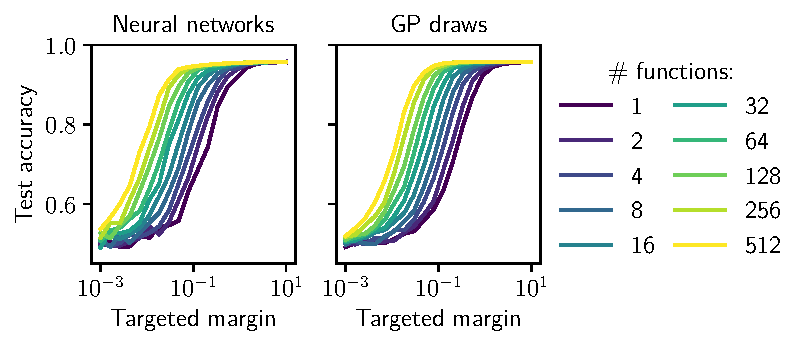
\includegraphics{figures/ensemble.pdf}
    \caption[Test accuracy as a function of normalised margin]{Test accuracy as a function of normalised margin, for both width-2048 neural networks (left) and neural network--Gaussian processes (right). The task was binary classification of MNIST digits \citep{lecun2010mnist} using a 5-layer multilayer perceptron. Each curve shows the test accuracy of the average over a number of functions, where each function in the average attains the specified value of normalised margin. The main behaviour visible is that one function of large normalised margin appears equivalent to the average of many functions of small normalised margin. The NNGP experiments used Equation \ref{eq:nngp-norm-margin} to control normalised margin. The neural network experiments controlled Frobenius-normalised margin by minimising square loss with respect to rescaled labels, and projecting every weight matrix to a hypersphere of fixed Frobenius norm at each iteration.}
    \label{fig:nn-margin}
\end{figure}\clearpage

\section{Empirical comparisons between classification strategies}

This section reports an experimental comparison of various binary classification strategies for both Gaussian processes and neural networks. The task was binary classification of MNIST digits \citep{lecun2010mnist} using a 7-layer relu multilayer perceptron. The width was set to either 1000 or infinity (via the neural network--Gaussian process correspondence).

For neural network--Gaussian processes, the classification strategies tested were:
\begin{enumerate}
    \item \textit{Gibbs classifier:} the sign of a random posterior sample.
    \item \textit{Bayes classifier:} the majority vote over the posterior.
    \item \textit{BPM classifier:} the sign of the minimum RKHS norm kernel interpolator.
\end{enumerate}
The spherised Gaussian process posterior (Definition \ref{def:gpc-posterior-spherised}) was used for reasons of computational tractability. Also, several generalisation bounds for Gaussian processes and kernel classifiers are plotted:
\begin{enumerate}
    \item \textit{Rademacher bound:} a uniform convergence bound for kernel classifiers \citep[Theorem 21]{rademacher}.
    \item \textit{Gibbs bound:} Inequality \ref{eq:sph-bound} of Theorem \ref{thm:pac-bayes-gpc}.
    \item \textit{BPM bound:} Inequality \ref{eq:k-pb3} of Theorem \ref{thm:k-bpm}.
\end{enumerate}

For finite width neural networks, the classification strategies considered were:
\begin{enumerate}
    \item \textit{Gibbs classifier:} train a randomly initialised network to fit the train sample to small Frobenius-normalised margin.
    \item \textit{Bayes classifier:} take the majority vote over 501 networks trained from different random initialisations to small Frobenius-normalised margin.
    \item \textit{BPM classifier:} train a randomly initialised network to fit the train sample to large Frobenius-normalised margin.
\end{enumerate}

The results for Gaussian processes and kernel classifiers are presented in
Figure \ref{fig:k-bpm}, while the results for neural networks are presented in Figure \ref{fig:nn-bpm}. The results support the idea that minimum RKHS norm kernel interpolators, and large Frobenius-normalised margin neural networks, are Bayes point machines.

\begin{figure}[p]
    \centering
    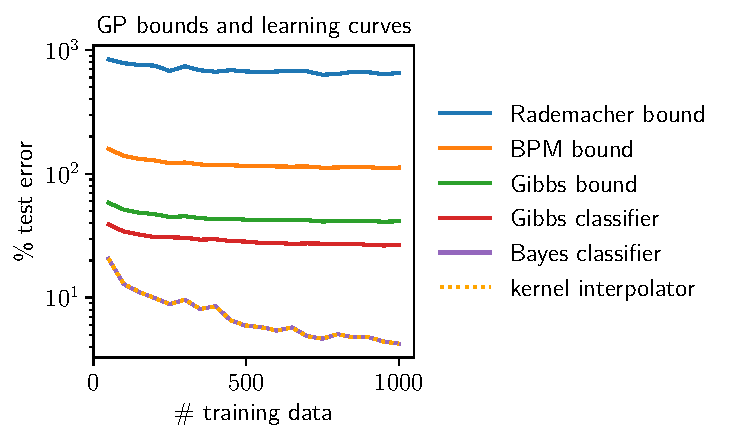
\includegraphics{figures/gp.pdf}
    \caption[Testing classification strategies for Gaussian processes and kernels]{Testing classification strategies for Gaussian processes and kernels, on an MNIST \citep{lecun2010mnist} binary classification task. The Bayes classifier and kernel interpolator attain indistinguishable performance, supporting the claim that minimum RKHS norm kernel interpolation is a Bayes point machine. Despite the kernel interpolator significantly outperforming the Gibbs classifier in practice, the order of the Gibbs and BPM bounds are reversed. Still, the BPM bound is substantially smaller than the Rademacher bound.}
    \label{fig:k-bpm}
\end{figure}
\begin{figure}[p]
    \centering
    \hspace{.25em}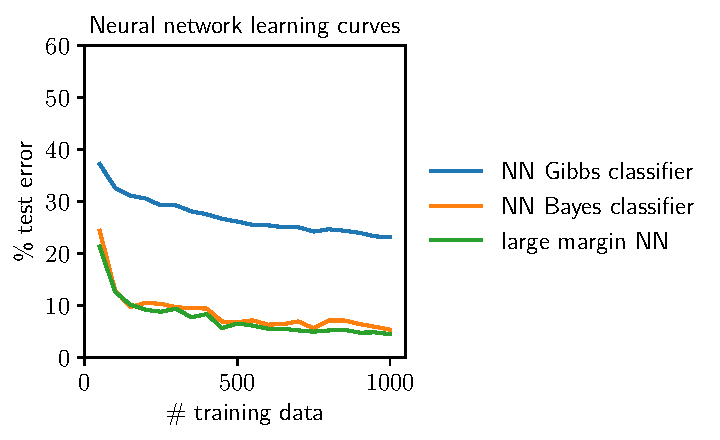
\includegraphics{figures/nn.pdf}
    \caption[Testing classification strategies for neural networks]{Testing classification strategies for neural networks, on the same task as Figure \ref{fig:k-bpm}. The Bayes classifier reports a majority vote over 501 small margin networks. It attains similar (though not identical) performance to a single neural network of large Frobenius-normalised margin. This supports the idea that large margin neural networks are Bayes point machines. Both classifiers substantially outperform the corresponding Gibbs classifier.}
    \label{fig:nn-bpm}
\end{figure}

\printbibliography[heading=subbibliography]
\end{refsection}